\documentclass{article}

% set font encoding for PDFLaTeX or XeLaTeX
\usepackage{ifxetex}
\ifxetex
  \usepackage{fontspec}
\else
  \usepackage[T1]{fontenc}
  \usepackage[utf8]{inputenc}
  \usepackage{lmodern}
\fi
\usepackage{graphicx}
% used in maketitle
\title{Actividad 3}
\author{Roberto Alexis Gomez Pintor}

% Enable SageTeX to run SageMath code right inside this LaTeX file.
% documentation: http://mirrors.ctan.org/macros/latex/contrib/sagetex/sagetexpackage.pdf
% \usepackage{sagetex}

\begin{document}
\maketitle
\section{Introduccion}
En esta actividad realizamos el uso de datos de sondeos atmosféricos de la Universidad de Wyoming, teniamos que elejir una estacion de un pais con las fechas del 22 diciembre y 22 de junio del 2017. Los datos los usaremos en Jupyter Notebook, ademas demeos obtener la graficas de Temperatura, temperatura del rocio, velocidad del viento y humedad relativa, ademas de manipular los datos en Phyton.

\section{Fundamentos}
Hasta finales de dicho siglo XIX y principios del XX, cuando surgen en todo el mundo las llamadas estaciones aerológicas, iniciándose y generando mediciones de los parámetros atmosféricos a diferentes alturas con ayuda de instrumentos que son elevados por medio de globos y cometas. El objetivo final era estudio de las capas bajas y medias de la atmósfera para trazar a diversas alturas las cartas sinópticas, necesarias para predecir el tiempo en dichas zonas.

\section{Analisis de datos}
Los datos se usaron fueron obtenidos de los sondeos atmosfericos de la universidad de Wyoming, los datos obtenidos fueron de una estacion en Rusia en la ciudad de Vologrado, debido a que en ambas fechas tanto diciembre y junio, muchas otras estaciones en ese año no tenian datos o faltaban,se elijio esta debido a que sus datos estaban bastante completos, esta falta de datos en las lineas de informacion causaba algunos errores que impedia un funcionamiento adecuado.

\section{Resultados}
Los resultados que se obtuvieron los analizaremos en las graficas posteriores referente a la temperatura y temperatura del rocio, la velocidad de los vientos medido en nudos y humedad relativa como funcion de la altura.

\begin{figure}
  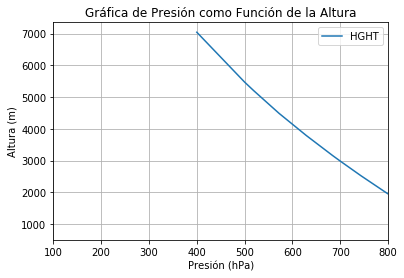
\includegraphics[width=\linewidth]{presiondic.png}
\end{figure}

\begin{figure}
  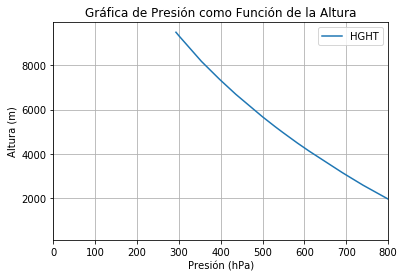
\includegraphics[width=\linewidth]{presionjun.png}
\end{figure}

\begin{figure}
  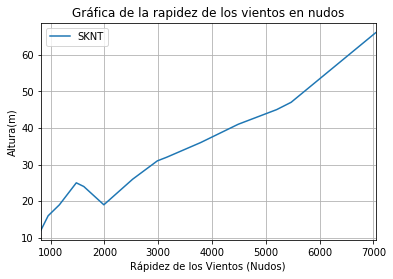
\includegraphics[width=\linewidth]{rapidezvientos.png}
\end{figure}

\begin{figure}
  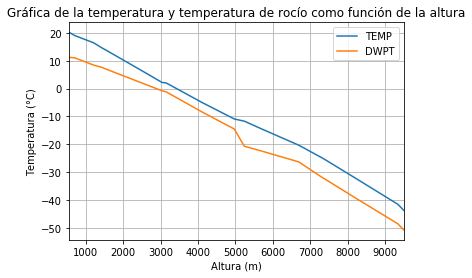
\includegraphics[width=\linewidth]{roctemp.png}
  \caption{Mes de Junio.}
\end{figure}

\begin{figure}
  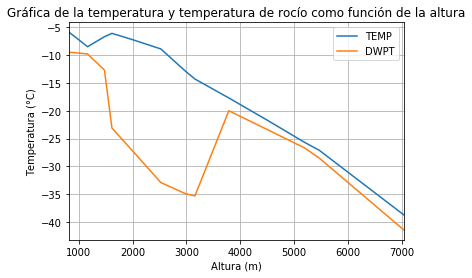
\includegraphics[width=\linewidth]{roctempdic.png}
  \caption{Mes de Diciembre.}
\end{figure}

\section{Conclusion}
A manera de conclusión es debe mencionar que la actividad se llevó a cabo con un grado de dificultad medio-bajo, debido a que se desarrollo el codigo mediante base otro para entender el proceso de que los datos se obtuvieron de la web dieran resultados para las graficas y ver sus conclusiones.

\section{Apendice}
\subsection{¿Cuál es tu opinión general de esta actividad?}
La actividad fue algo bastante similar a la anterior dando el cambio principal fue donde obtuvo los datos para trabajo, haciendo que sea relativamente sencillo trabajar.
\subsection{¿Qué fue lo que más te agradó? ¿Lo que menos te agradó?}
La gran variedad de datos en diferentes entre las estaciones me parecio bastante y completa, lo que no fue mi agrado varias estaciones que encontretenian datos que faltaban.
\subsection{¿Que consideras que aprendiste en esta actividad? }
EL manejo de datos para usarlos en Jupytter pero enves de trabajar con un conjunto de informacion, seria trabajar con diferentes de estos conjuntos con diferentes fechas.
\subsection{¿Qué le faltó? ¿O le sobró? }
Pues no he encontrado nada que faltara o sobrara.
\subsection{¿Que mejoras sugieres a la actividad?}
Nada, me parece que la actividad esta bastante bien hecha y definida.

\end{document}
